\documentclass[12pt]{scrreprt}

%\usepackage[
%HomeHTMLFilename=index,     % Filename of the homepage.
%%HTMLFilename={node-},       % Filename prefix of other pages.
%%IndexLanguage=english,      % Language for xindy index, glossary.
%latexmk,                    % Use latexmk to compile.
%%   OSWindows,                  % Force Windows. (Usually automatic.)
%mathjax,                    % Use MathJax to display math.
%]{lwarp}


\usepackage{graphicx}
%\usepackage{subcaption}
\usepackage{float}
%\usepackage[nottoc,numbib]{tocbibind}
\usepackage{caption}
\usepackage[backend=bibtex]{biblatex}% Sort by citation order

\addbibresource{references.bib}


%\newcommand{\email}[1]{\texttt{\href{mailto:#1}{#1}}}

%\title{ENGR 446: Milestone Report I: Project Background}
%\author{David Li\footnote{Undergraduate student, Department of Electrical and Computer Engineering, University of Victoria, \email{lidavid@uvic.ca}}}

%\makeatletter
%\let\inserttitle\@title
%\let\insertauthor\@author
%\makeatother


%% Print Title Page
\makeatletter
% Create \printauthor command which will display contact info                     
\def\printauthor{%                  
	{\large \@author}}              
\makeatother
% Honestly, if footcite works that would be adequate for me
\author{%
	\textbf{Name: }  David Li \\
	\textbf{Student Number:} V00818631	\\
	\textbf{Year}  Fourth Year Student  \\
	\textit{Discipline:} Computer Engineering \\  \vspace{4pt}
	\textit{Email:} \href{mailto:lidavid@uvic.ca}{lidavid@uvic.ca}
}

%\bibliography{references.bib}

\usepackage[table]{xcolor}
\usepackage{tabularx}		% Tabulars with adjustable-width columns
\definecolor{lightgoldenrodyellow}{rgb}{1, 0.93, 0.55}
\definecolor{firebrick}{rgb}{0.7, 0.13, 0.13}
\definecolor{gray}{rgb}{0.5, 0.5, 0.5}
\definecolor{almostWhite}{rgb}{0.95, 0.95, 0.95}
\definecolor{purpleMix}{rgb}{0.35, 0.07, 0.57}
\newcommand*{\arraycolor}[1]{\protect\leavevmode\color{#1}}
\newcolumntype{A}{>{\columncolor{blue!50!white}}c}
%\newcolumntype{B}{>{\columncolor{lightgoldenrodyellow}}c}
\newcolumntype{B}{>{\columncolor{purpleMix!75}}c}
\newcolumntype{C}{>{\columncolor{firebrick!50}}c}
\newcolumntype{D}{>{\columncolor{lightgoldenrodyellow}}c}
\newcolumntype{E}{>{\columncolor{white!60!purple!20!green!20}}c} 

\newcommand{\foo}{\color{blue}\makebox[0pt]{\textbullet}\hskip-0.5pt\vrule width 1pt\hspace{\labelsep}}

\usepackage{kpfonts}	    % Fonts used in the title page

\newcommand{\onlineCite}{[Online] Available: }	% Used in BIBLIOGRAPHY

\usepackage{tikz}

\usepackage{url}
\makeatletter
\g@addto@macro{\UrlBreaks}{\UrlOrds}
\makeatother

% Fancy example listings from https://tex.stackexchange.com/questions/212943/fancy-example-environment
\usepackage{chngcntr}
\usepackage[tikz]{mdframed}


\definecolor{greentitle}{RGB}{61,170,61}
\definecolor{greentitleback}{RGB}{216,233,213}

\newcounter{mdexample}
\counterwithin{mdexample}{section}

\newenvironment{myexample}[1]
  {\stepcounter{mdexample}\begin{mdframed}[
    frametitle=#1,
    frametitlefont=\normalfont,
    topline=false,
    bottomline=false,
    rightline=false,
    linecolor=greentitleback,
    linewidth=2pt,
    singleextra={
      \node[
        overlay,
        outer sep=0pt,
        anchor=north east,
        text width=2.5cm,
        minimum height=4ex,
        fill=greentitleback,
        font=\color{greentitle}\sffamily\scshape
      ] at (O|-P) {example~\themdexample};
      },
    firstextra={
      \node[
        overlay,
        outer sep=0pt,
        anchor=north east,
        text width=2.5cm,
        minimum height=4ex,
        fill=greentitleback,
        font=\color{greentitle}\sffamily\scshape
      ] at (O|-P) {example~\themdexample};
      }
    ]
  }
  {\end{mdframed}}
\newcommand\Solution{\par\textbf{\textsf{Solution}}\par\medskip}


\usepackage{hyperref}

\usepackage[titletoc]{appendix}	%% appendix will be in the toc
% What I want is References and subsections or paragraphs 

\usepackage{breakurl}
\begin{document}

\makeatletter
% Create \printauthor command which will display contact info                     
\def\printauthor{%                  
	{\large \@author}}              
\makeatother
\author{%
	David Li \\
	V00818631	\\
	%Term 3B \\
	Computer Engineering \\  
	%\vspace{4pt}lidavid@uvic.ca 
}

%\maketitle

% Picture from https://pixabay.com/en/blockchain-block-chain-technology-3019120/

\begin{titlepage}
 \begin{tikzpicture}[remember picture, overlay]
  \node[opacity=0.05,inner sep=0pt] at (current page.center)
   {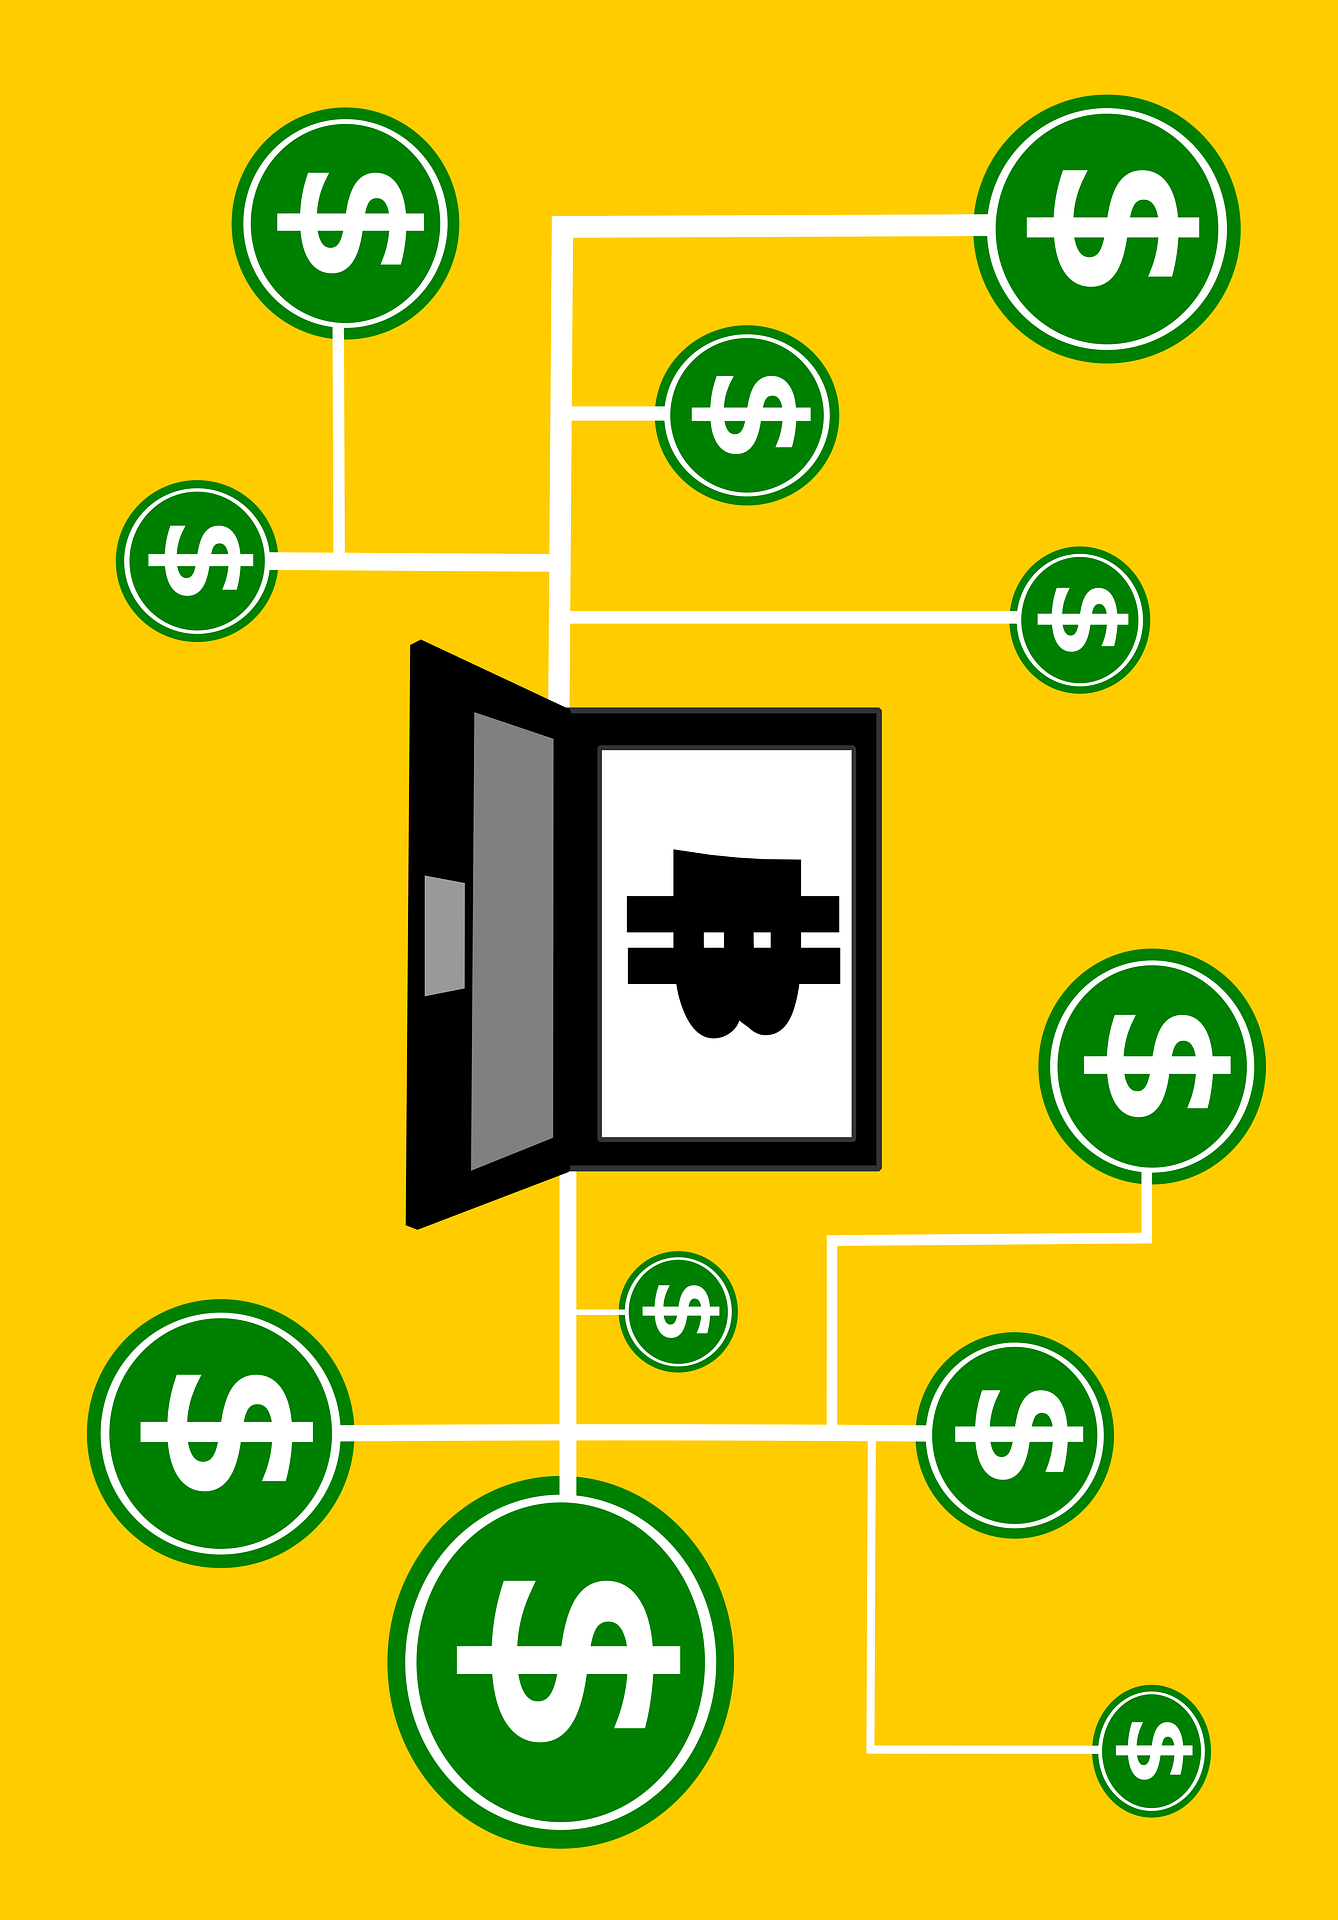
\includegraphics[width=\paperwidth,height=\paperheight]{bchainCOol.png}};
  \end{tikzpicture}
	\begin{center}
		{\vspace*{3pt} }
		{\Large University of Victoria \\ \vspace{4pt}}
		{\Large Faculty of Engineering \\ \vspace{4pt}}
		{\Large ENGR 446: Milestone Report II: Engineering Analysis \\ \vspace{4pt}}  
		\rule[13pt]{1\textwidth}{1pt} \\ \vspace{1pt}
		{\LARGE \textbf{{Simplification of Transactions by leverage blockchain technologies and smart contracts}} \\ \vspace{15 pt}}
		
		{\Large David Li \hfill Computer Engineering \hfill  V00818631 }
		%{\Large BC Ministry of Transportation and Infrastructure \\} 
		%					\vspace{4pt}} 
		%{\Large Information Management Branch}
		%	\vspace{4pt}}
		%{\Large Victoria, British Columbia, Canada \\ \vspace{60pt}}
		%\AddToShipoutPicture*{\BackgroundPic}
	%	\vspace{10pt}
		%\begin{minipage}

		%{\vspace{60pt} \\}
		%{\vspace{60pt}}
		{\vspace*{-20pt}}
		\begin{figure}[htb]
		\centering
		\makebox[0pt][c]{%
		\begin{minipage}{0.59\linewidth}
		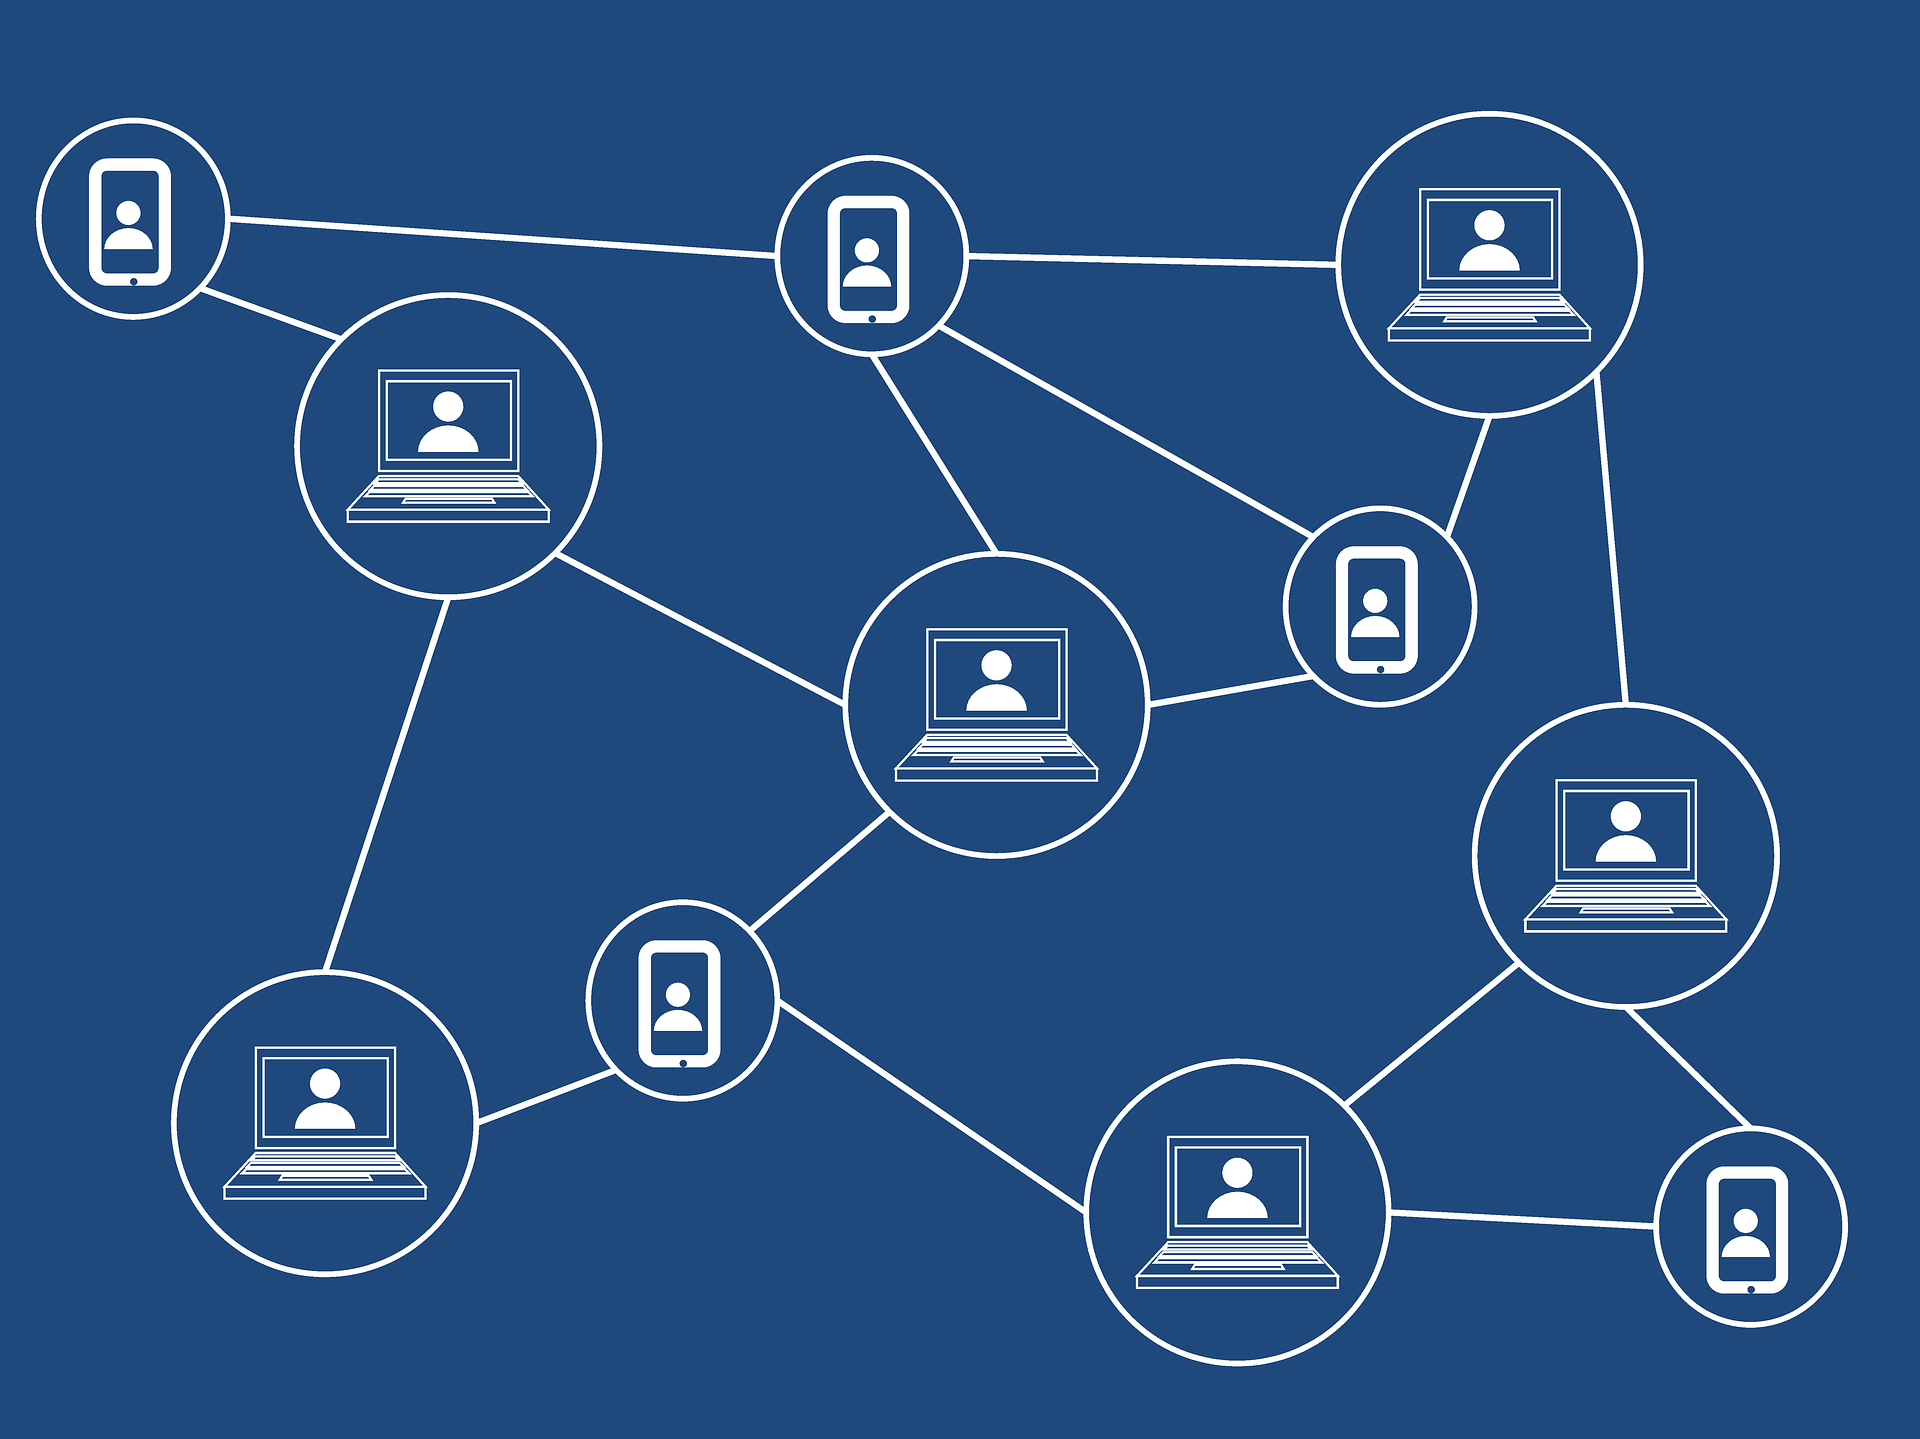
\includegraphics[width=1\linewidth,%
		  		keepaspectratio]{bchain.png}
		\end{minipage}
		\begin{minipage}{0.59\linewidth}
		
\includegraphics[width=1\linewidth,%
				  keepaspectratio]{bitcoinImageTrans.png}
		\end{minipage}%
		}%
		\end{figure}
%		\begin{minipage}{0.96\linewidth}
%			\begin{flushright}
%				\printauthor
%			\end{flushright}
%		\end{minipage}
%		\begin{minipage}{0.02\linewidth}
%			\rule[0pt]{1pt}{70pt} 
%		\end{minipage}

	%	\vspace{40pt}
		{\Large \today \\ \vspace{10pt}}
			{\Large In partial fulfillment of the academic requirements of this academic course}
	\end{center}%	\AddToShipoutPicture*{\fpict}
\end{titlepage}

\renewcommand{\contentsname}{Table of Contents}
\tableofcontents
\listoffigures
\listoftables

\newpage 

\chapter{Proposed approach}

Leveraging the largest public blockchains with smart contracts, grants enough computation power 
for quick transactions, while keeping transparency as a high priority. Reliability of decentralized applications is significant provided users are incentivized to support the shared network.

 	\begin{figure}[ht]
  	\centering 
  	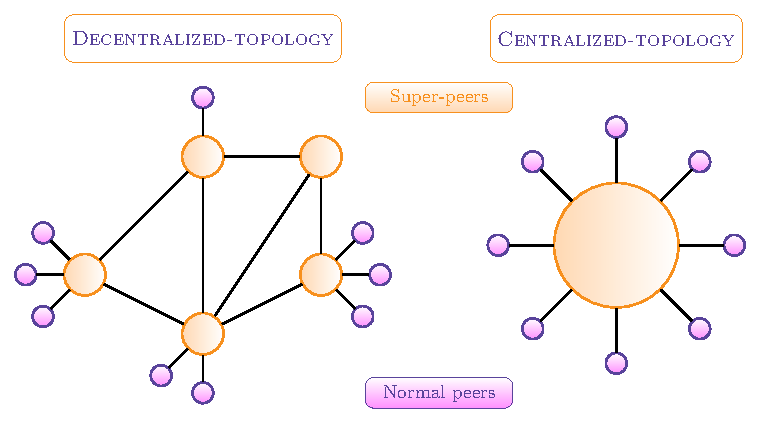
\includegraphics[width=1\linewidth]{ms-II/DappVApp.pdf}
  	\caption{Decentralized and centralized topology}
  	\label{toplogy}
  	\end{figure}
  	
  	 Comparing the process of purchasing a home with and without smart contracts will illustrate its simplicity and efficiency. Since the cost of transactions (gas) on ethereum is relatively low \cite{ethereumWhitePaper:Online} and replicating software costs practically nothing, development is the foremost financial burden.   Furthermore, cutting out the middlemen in this process (lawyers and real-estate agents) greatly reduces the financial burden while increasing transaction speed and transparency.
  	
  	\section{Project Plan}
 	\begin{figure}[ht]
   	\centering 
   	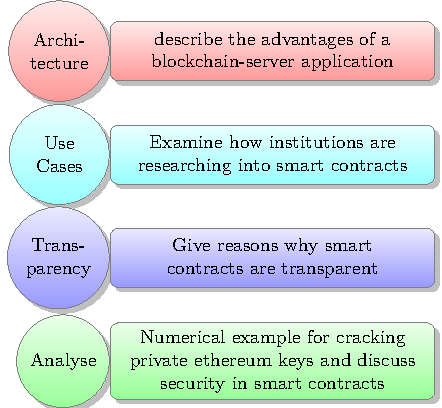
\includegraphics[width=1\linewidth]{ms-II/smartDiagramProjectPlan.pdf}
   	\caption{Smart Diagram for proposed approach}
   	\label{toplogy}
   	\end{figure}
   	 	Creating decentralized applications is challenge because technologies are nascent, undergoing evolution and tools are in infancy.


\chapter{Engineering Analysis}

\section{Advantages and Disadvantages of Decentralization }
Currently, centralized IT systems are vulnerable to "malicious attacks, software and hardware faults, human mistakes (e.g., software and hardware misconfigurations") \cite{5936160}. Decentralized systems have no single point of failure, improved security and are more transparent, however, efficient code is more important in smart contracts. As illustrated in \ref*{fig:DApp} a blockchain-server architecture model allows for developers to implement decentralized applications with smart contracts while maintaining the flexibility and simplicity of retrieving and sending information.
 
\begin{figure}[ht]
%\begin{adjustbox}{center,max width=1.1\textwidth}
\centering
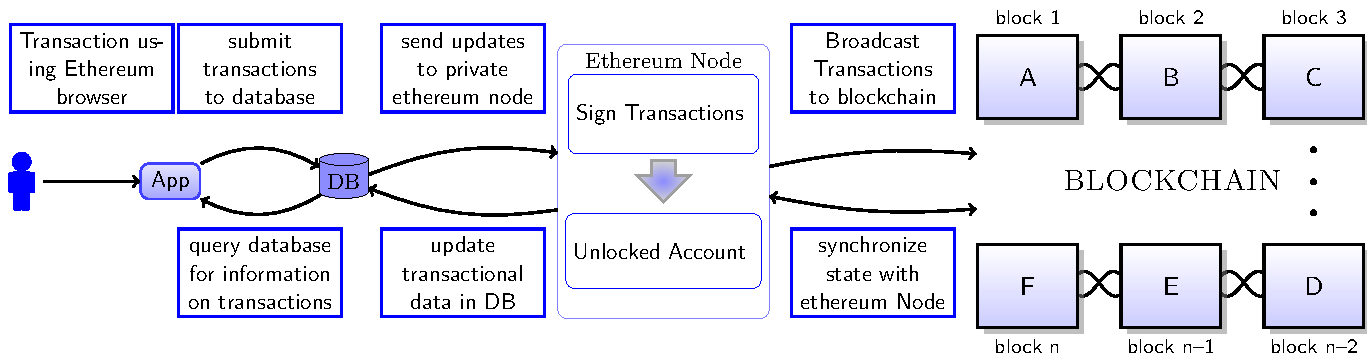
\includegraphics[width=1\linewidth]{ms-II/blockchainInSimpleApp.pdf}
%\end{adjustbox}
\caption{An example of server-blockchain architecture in a DAPP.}
\label{fig:DApp}
\end{figure}
Usage on blockchain technologies is actively being explored in medical research \cite{pmid28357041} more transparency, real-estate and supply chains.
Despite, the obvious advantages of decentralized and blockchain technologies,  a lack of resources for unpopular materials may result in prolonged downloads. An equivalent anecdote is a inadequately seeded torrent results in intolerable download speeds.  Whereas a traditional database only checks, writes and stores data once, a decentralized blockchain system require thousands of operations to write and store data, therefore the costs of maintaining a blockchain are substantial higher and only justifiable with increased utility/security \cite{EthScale:Online}. 

 \section{Security of Smart Contracts}
 
 Blockchain transactions are secure because that are immutable and decentralized. However, exploiting bugs in smart contracts are financially devastating \cite{funnyJoke:Online} as fraudulent transactions cannot be reverted. Disconnects between software developers and security experts has resulted in 3 out of 4 "applications produced by software vendors fail to meet OWASP Top 10 standards" \cite{veraCode:Report}. Although blockchain technologies increase underlying security and reliability, exploiting poorly coded and insecure smart contracts remains a major risk, and releasing open-source code allows hackers exploit flaws in the codebase before corrective processes are applied.  



\subsection{Brute force cracking of private keys}
A ethereum key, which is randomly selected 256 digits \cite{ethereumWhitePaper:Online}, is very difficult to hack. A simple calculation illustrates the impracticalities of brute forcing for a 256 bit key. Assuming that a 1 exaflop ($10^{18}$ calculations per second) 15 megawatts supercomputer \cite{Service617} is used, electricity costs are 0.1326 per kWH \cite{BCHydroRates}. % In order to hack a 256 bit key by brute force $2^{256}$ decryptions are required. Powering the machine costs \$ 1.989 million excluding maintenance and hardware costs. It can perform
\vspace*{-0.1cm}
\begin{align}
& 2^{256} = 1.1569 \times 10^{77} \text{decryptions} \\
& 10^{18} \frac{\text{decryptions}}{\text{second}} \times \frac{3.154 \times 10^7 second}{1 year} = 3.154 \times 10^{25} \frac{\text{decryptions}}{year} \\
& \text{Number of machines} = \frac{1.1569 \times 10^{77} }{3.154 \times 10^{25} } \text{years}= 3.66804 \times 10^{51} years
%So in order to brute force hack a private key in a year 
\end{align}

 	\begin{figure}[ht]
  	\centering 
  	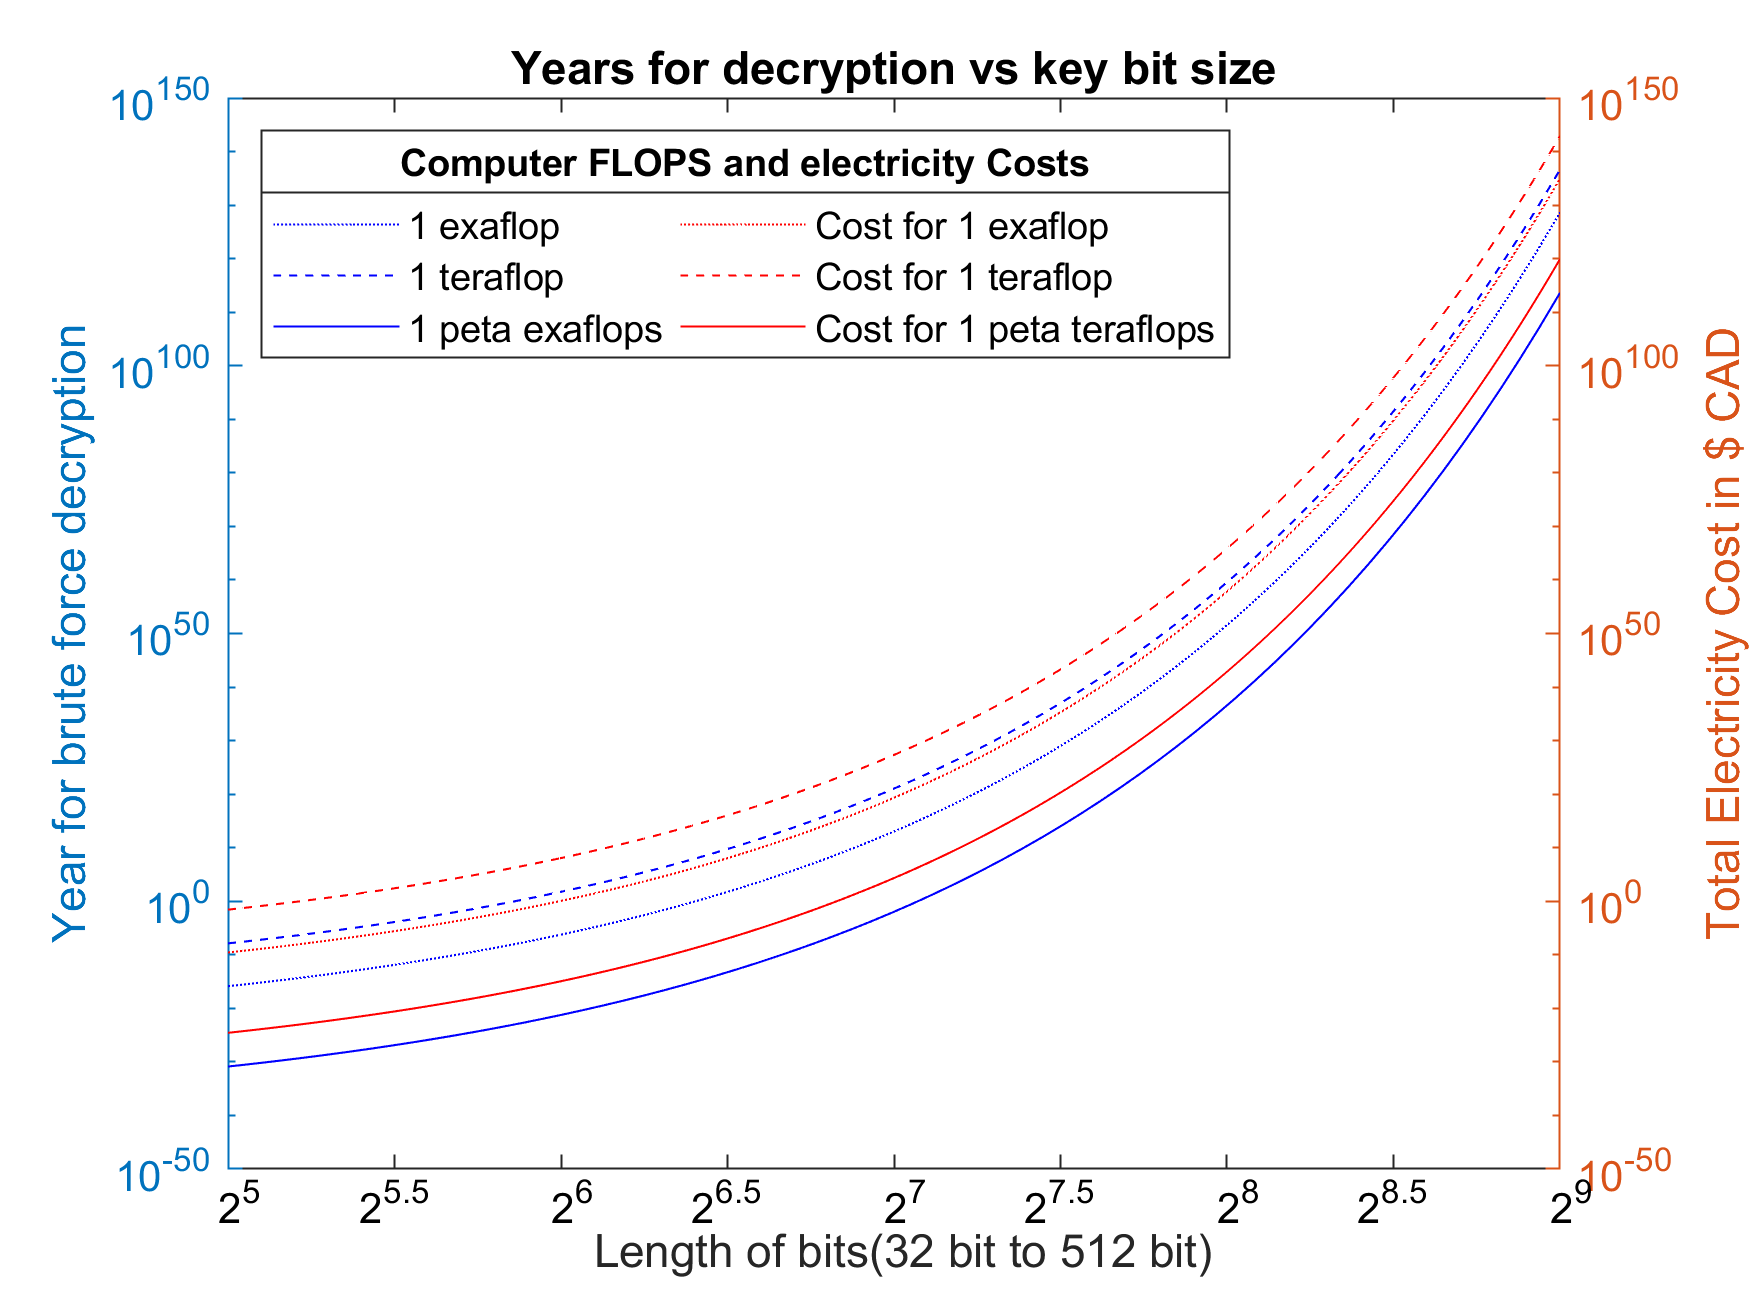
\includegraphics[width=0.7\linewidth]{matlab/epicPic.png}
  	\caption{Difficulty of brute forcing a 256-bit key}
  	\label{security:fig2}
  	\end{figure}
 
%This would cost $1.989 \times 10^6 \frac{\$ CAD}{year} \times 3.66804 \times 10^{51} years = \$ 7.2957 \times 10^{57}$. This amount of money is impractical for anyone to spend.
 	
 	
 \subsection{Considerations for Quantum computing}
 As shown in \ref*{security:fig2}, if powerful quantum (1 peta teraflops) computers become commonplace existing 128 bit ($2^7$) are easily hacked and 256 bit ($2^8$) are insecure. According to the the Margolus–Levitin theorem processing power of computer can reach $6 \times 10^{33}$ operations per second per joule. This indicates that existing 128 bit keys and even 256 bit keys are unsecure in a quantum computing age. 
 
 % add section for high end gaming computer
 %lthough, finding prime factors is not possible on traditional computers with a bit being 0 or 1, 
 %If quantum computers become commonplace, the usage of quantum algorithms such as https://en.wikipedia.org/wiki/Shor's\_algorithm allow a computer to quickly find prime factors and would break public-key cryptography. In addition, the limit of quantum computation as stated by the Margolus–Levitin theorem where inputting 1 Joule to a computer can never "increase its processing rate by more than about $3 \times 10^{33}$ operations per second" \cite{MARGOLUS1998188}.
 
 % https://en.wikipedia.org/wiki/Margolus%E2%80%93Levitin_theorem
 
 \subsection{Cheaper and Faster Transactions}
 Typically, transactional costs are be categorized broadly as: \cite{RePEc:ucp:jlawec:v:22:y:1979:i:1:p:141-62}
 % @ARTICLE{RePEc:ucp:jlawec:v:22:y:1979:i:1:p:141-62,
% title = {The Problem of Externality},
% author = {Dahlman, Carl J},
% year = {1979},
% journal = {Journal of Law and Economics},
% volume = {22},
% number = {1},
% pages = {141-62},
% url = {https://EconPapers.repec.org/RePEc:ucp:jlawec:v:22:y:1979:i:1:p:141-62}
% }
 \begin{itemize}
 \item Search and information costs (determining what is the suitable goods that is available on the market)
 \item Bargaining costs (costs to come to acceptable agreement)
 \item policing and enforcement costs (making sure other party sticks to term of contract)
 \end{itemize} 
 
 Usage of smart contracts practically eliminate policing and enforcements costs as transactions are dictated by code, bargaining costs are reduced since the middlemen are removed, and reliable, immutable information on current and previous transactions are publicly displayed on the blockchain. Deploying a smart contract is inexpensive, however any changes in source code require the contract redeployment.
 
 \begin{figure}[ht]
   	\centering 
   	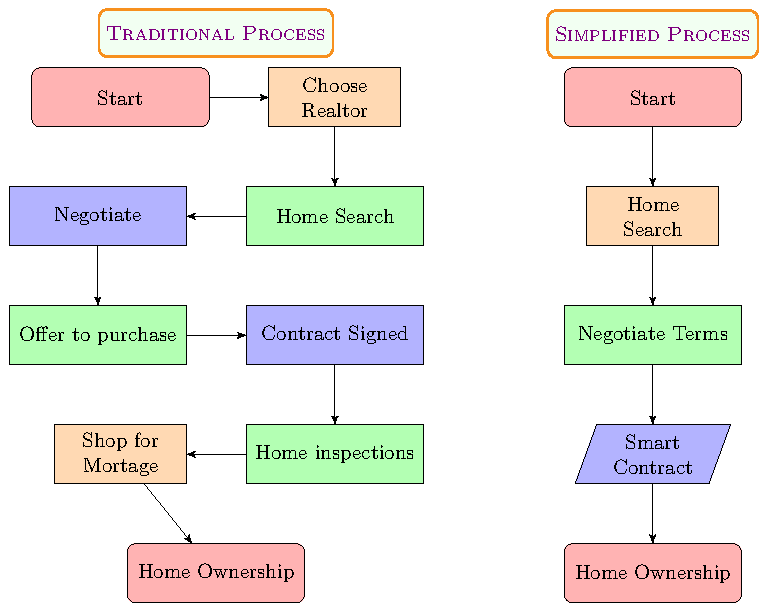
\includegraphics[width=0.7\linewidth]{ms-II/simplifyingPurchasingAHome.pdf}
   	\caption{Flow Chart illustrating how smart contracts can simplify buying a home}
   	\label{smartContract}
   	\end{figure}
   	
As specified in \cite{buyingHome:Online}, the process of purchasing a home can take up to a month, however by using smart contracts, friction between parties will be reduced, the transactions are more transparent and occur much quicker.  Writing data to the blockchain is slower than a traditional database, however usage of side-chains (separate blockchain that enables fast transactions without clogging up the main network) can greatly reduce transaction completion time \cite{sideChains:Online}. For instance, inserting information info a database is an order of magnitude in milliseconds, but writing to the blockchain requires a order of magnitude in seconds. 

%Writing information to the blockchain is significantly slower than a traditional database, however, with side chains 
%A traditional centralized database only needs to be written to once. A blockchain needs to be written to thousands of times. A traditional centralized database needs to only checks the data once. A blockchain needs to check the data thousands of times. A traditional centralized database needs to transmit the data for storage only once. A blockchain needs to transmit the data thousands of times.

%The costs of maintaining a blockchain are orders of magnitude higher and the cost needs to be justified by utility.
\chapter{Discussion}


Decentralized systems are inherently more reliable, resilient against brute force attacks, and are more transparent. Even though immutable and irreversible transactions are advantageous, criminals leverage cryptocurrencies for illegal transfer of funds. This implies the ability to undo fraudulent or criminal activity is extremely important, but reversible transactions is an anti-pattern. For example EOS, a centralized blockchain platform, was criticized for freezing accounts without due process and community backing. \cite{EOS:Online}. In addition, centralized systems require users to trust vendors and oftentimes personal data usage lacks transparency. Currently, research into blockchain technologies are actively researched that can disrupt existing industries including finance, real-estate and supply chains. \hfill \break
% 



Smart contracts are useful because that cannot be changed by the parties involved in the transactions, yet, in some cases such as criminal activity, the ability to reverse transactions or freeze accounts is extremely desirable.
Deployment of a smart contract is inexpensive, however, development and maintenance costs for blockchain applications can be costly. This implies that transaction expenses decrease significantly, but running a blockchain node, ensuring high quality code for smart contracts is challenging and expensive. Decentralized applications are transparent because information is available in the publicly ledger and parties participating in a transaction cannot alter it. Overcomplicated code and bugs in smart contracts are severely detrimental because of malicious transactions by scammers or hackers. \hfill \break


As shown in Figure \ref{smartContract}, smart contract reduce complexity of transactions allowing buyers to directly interact with sellers. This illustrates how useful smart contracts are, but lack of legislation for blockchain technologies, consortiums unwilling to adopt decentralized applications (may prefer private blockchains), and ability for hackers to exploit bugs suggest transactions governed by code is decades away. Solutions to existing problems in blockchain technologies such as latency, immutable transactions and widespread acceptance by consortiums are addressed through innovations such as sidechains, centralized blockchain platforms like EOS and private blockchains infrastructure. \hfill \break


Overall, blockchain technologies allow for users to have a unique digital presence, securely transfer ownership of assets and avoid key shortcomings of centralized IT systems.
\printbibliography

\begin{appendices}
\chapter{Project Background}
\section{Background}

In 2008 bitcoin white paper [1] described a way to solve the double spending problem without a centralized body using blockchain. Although, the value of bitcoin (BTC) has grown exponentially, high computational and energy consumption in mining and slow performance [2].  Released in July 30, 2015, Ethereum, an open-source platform based on blockchain technology, distinguishes itself from bitcoin through faster transactions, unlimited processing capability for {smart contract}, and its network is optimized to support Decentralized Applications [3].

%modify this for markdown file
\begin{table}[ht]
\centering
\renewcommand\arraystretch{1.4}\arrayrulecolor{blue}
%\captionsetup{singlelinecheck=false, labelfont=sc, labelsep=quad}
\caption{Timeline of Cryptocurrency}%\vskip -1.5ex
% lwarp table, and print edition (uncomment stuff below for good copy)
%\begin{tabular}{l l }%
% Good copy for print edition
\begin{tabular}{@{\,}r <{\hskip 2pt} !{\foo} >{\raggedright\arraybackslash}p{5cm}}
\toprule
%\addlinespace[1.5ex]
2008 & Bitcoin White Paper \\
2009 & Bitcoin Genesis Block\\
2013 & 1 BTC = \$ 31 USD\\
2013 & Ethereum White Paper \\
2015 & Ethereum Genesis Block\\
2015 & HyperLedger starts \\
2017 & Over 1000 different cryptocurrencies \\
2018 & AWS Blockchain Templates \\
\end{tabular}
\end{table}


Blockchain technology is revolutionizing the internet by establishing trust in shared data. [3].
	Additionally, transactions recorded on the blockchain are practically impossible to remove or change. 
	A decentralized application, or DApp are deployed on peer to peer networks such as Ethereum or on the cloud.
	
	
Traditional legal contracts are written to represent the contracting parties. In a smart contract, self-executing source code is used to automatic transactions that are publicly available on the blockchain [3].

\begin{figure}[ht]
		\centering
		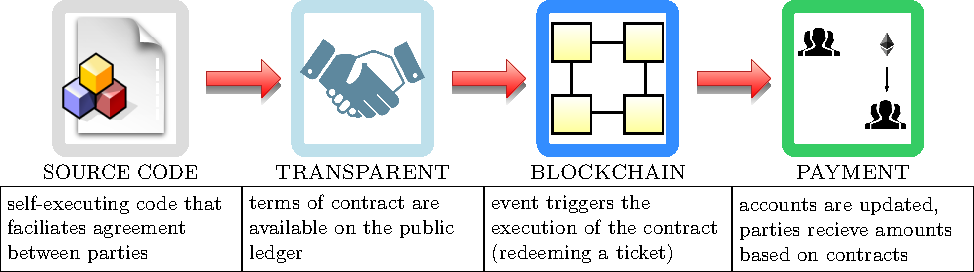
\includegraphics[width=1\linewidth]{smartContractsExp.pdf}
		\caption{Illustrating how a smart contract works}
		\label{fig:smartContracts}
\end{figure}

\newpage 

\section{Objective}
The prominence of cryptocurrency and decentralized applications suggests usage of smart contracts will experience explosive growth.

\subsection{Problem}

Currently commonplace transactions require days to process and for parties verify correctness. For example to purchase houses, a plethora of steps are required, one must interactive with lawyers, real-estate agents, home inspector, buy insurance and shop for a mortgage. 

\subsection{Purpose}
Leveraging existing blockchain technologies can automatic the majority of steps and cut out the middlemen, resulting in buyers conversing directing with sellers.
% Although smart contracts have immense potential to simplify transactions, issues such as limiting access to information, latency when updating (takes 10 minutes to write info to bitcoin blockchain), and immutability of translations (cannot undo transfer of assets) must be addressed.
% See https://www.cs.auckland.ac.nz/research/groups/ssg/homepages/yu-cheng/ytu001_PhDThesis.pdf
% https://researchspace.auckland.ac.nz/handle/2292/22092
\subsection{Aims}
The aims of this project are to develop a decentralized blockchain system that:
\begin{enumerate}
\item Reduce cost of transactions by at least 50\% from removing middlemen.
\item Improve transparency in software systems through augmented accessibility and understandability.
\item Has increased reliability and more secure than traditional systems.
%1. Uses 15% less material to decrease cost and weight.
%2. Has improved efficiency by reducing the air gap by 10%.
%3. Has no reduction in its reliability or increase in its maintenance requirements. 
\end{enumerate}
\subsection{Limitations}

The regulatory uncertainty and impact of future regulations on blockchain technologies such as smart contracts will not be investigated. In addition, criminal usage of cryptocurrencies to avoid taxation and legal repercussions are beyond the scope of this report. 
%The performance of the linear generator in extreme storm events will not be investigated as this
%cannot be accurately modeled using Airy linear wave theory. This project will be based on
%numerical simulations; no physical model will be tested to validate the results.

\newpage  
\section{Potential Solutions}

\begin{itemize}
	\item[---] \textbf{Public blockchains} are large distributed networks that are run through a native token such as bitcoin or ether. Anyone can participate and the community maintains its open-source code. The two largest public blockchains are Ethereum and Bitcoin. They are open for anyone to participate at any level and have open-source code that their community maintains.
	% rewrite and add section about composer
	\item[---] \textbf{Permissioned blockchains} define role based access control for individuals in the network and uses native tokens.  HyperLedger Composer, an open-source framework for permissioned blockchains, is used for smart contracts and for blockchain application development [4]. One use case is an accounting system that calculates payment, while hiding that information from unrelated organizations.  \hfill \break % Their core code may or may not be open source.
	\begin{figure}[ht]
	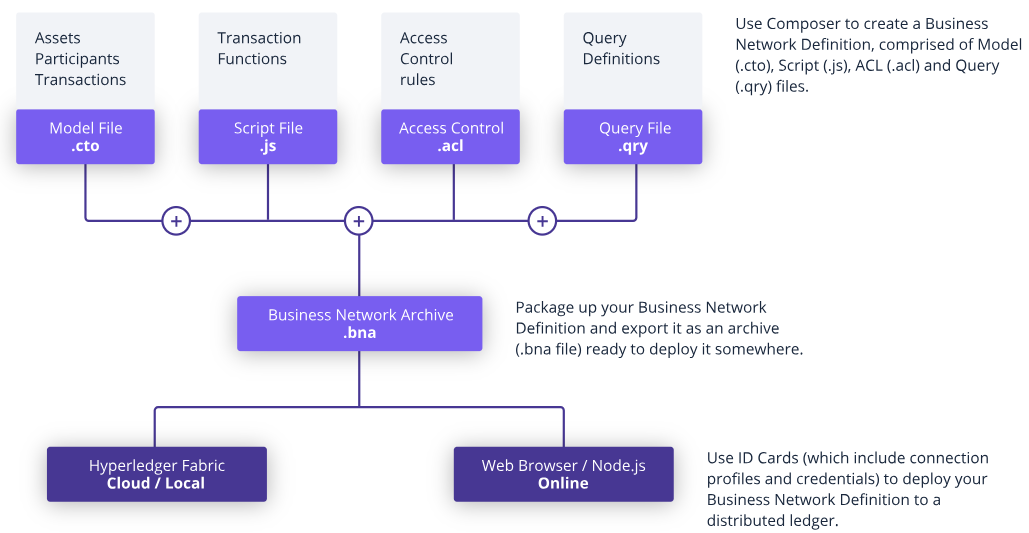
\includegraphics[width=1\linewidth]{composer-arch.png}
	\caption{Architecture of Hyperledger composer}
	\end{figure}
	\item[---] \textbf{Private blockchains}  membership is tightly controlled and lacks a native token. Useful for consortiums with trusted associates and exchanging confidential information, however, less powerful because it is supported by limited private resources. Large organizations such as governments will likely use these extensively.
\end{itemize}

\newpage 
\section{Initial Assessment}
% Discuss how it is significantly more accessible for money to issue their own currencies, ICOs

% Explain how much it costs to how a bunch, like 5%, getting an automatic system will be cheaper as wages will not be paid, cover cost of gas
% "Gas" is the name for a special unit used in Ethereum. It measures how much "work" an action or set of actions takes to perform: for example, to calculate one Keccak256 cryptographic hash it will take 30 gas each time a hash is calculated, plus a cost of 6 more gas for every 256 bits of data being hashed. Every operation that can be performed by a transaction or contract on the Ethereum platform costs a certain number of gas, with operations that require more computational resources costing more gas than operations that require few computational resources.

% https://ethereum.stackexchange.com/questions/3/what-is-meant-by-the-term-gas

Determining which platform is best for smart contracts should be done using a weighted decision matrix, based on the particular application. For internal processes such as supply chains, a private blockchain makes sense (data cannot be changed) and cryptographic auditing with known identities (public keys). For a trustless system that verifies every transaction, using a public blockchain is essential. In comparison, role-based access control is feasible by using a permissioned blockchain. \hfill \break
%\hfill \break 

Despite the slow speed of the public blockchain, innovations such as side chains enable quick transactions and are used in decentralized game development [5]. A permissioned blockchain allows role based access control which is essential in business applications. One example is to prevent unrelated parties from viewing other's data. 	Furthermore, smart contracts allow buyers and sellers exchange money, property, shares, or anything of value in a transparent, conflict-free way while avoiding the services of a middleman. This allows validation of complex transactions swiftly while maintaining transparency.
%modify this for markdown file

\begin{table}[H]
\centering
\caption{Sample Decision Matrix for designing a blockchain system}
\arrayrulecolor{white}
\arrayrulewidth=1pt
\renewcommand{\arraystretch}{1.5}
\rowcolors[\hline]{3}{.!50!white}{}
\begin{tabular}{D E A B C }
\multicolumn{1}{l}{}      & \multicolumn{1}{c}{Existing Systems}    & \multicolumn{3}{c}{BlockChain Systems}                                                                                    \\
\multicolumn{1}{c}{Criteria}                 & \multicolumn{1}{c}{Centralized} & \multicolumn{1}{c}{Public} & \multicolumn{1}{c}{Permissioned} & \multicolumn{1}{c}{Private} \\
speed and latency         &    5                                     &      7                                 &         7                                    &                  6                     \\
scalability         &        5                                &     9  8                                &          7                                &                         4               \\
security and immutablity  &     3                                    &                        7               &    8.5                                         &                   9                     \\
storage capacity          &        4                                 &            9                           &                         9                    &         6                               \\
transparency              &   3                                      &                         9              &    7                                            &               5                         \\
\multicolumn{1}{c}{Total} &    21                                     &               41.6                        &    38.5                                         &          30                             
\end{tabular}
\end{table}

 A decentralized system (peer to peer) has many advantages over a conventional centralized network including no single points of failure, cheaper distribution (servers are expensive), faster upload speeds and improved security. In addition, irreversible and immutable transactions are both an advantage and disadvantage. For example, an amateur coder killed the contract that allowed users to transfer Ether for the Parity Ethereum Wallet, rendering 150 to 300 million dollars completely useless [6].
Overall, the public blockchain with access to substantial collective resources is most viable in terms of scalability and transparency, however, institutes may prefer implementing permissioned or private blockchains internally for extended security and privacy. 


\newpage 
% Add survey of functionality, what industries could be impacted A survey of potential users. 
%\printbibliography

%\hypertarget{refs}{}

\section*{References for Appendix}

\hfill \break 


\leavevmode\hypertarget{ref-bitcoinWhitePaper:Online}{}%
{[}1{]} "Bitcoin white paper." \url{https://bitcoin.org/bitcoin.pdf}.

\leavevmode\hypertarget{ref-bitCoinProblems:Online}{}%
{[}2{]} S. Elnaj, "The problems with bitcoin and the future of
blockchain."
\url{https://www.forbes.com/sites/forbestechcouncil/2018/03/29/the-problems-with-bitcoin-and-the-future-of-blockchain}.

\leavevmode\hypertarget{ref-ethereumWhitePaper:Online}{}%
{[}3{]} "Ethereum white paper."
\url{https://github.com/ethereum/wiki/wiki/White-Paper}.

\leavevmode\hypertarget{ref-hyperledgerComposer:Online}{}%
{[}4{]} "Hyperledger composer overview."
\url{https://www.hyperledger.org/wp-content/uploads/2017/05/Hyperledger-Composer-Overview.pdf}.

\leavevmode\hypertarget{ref-loomNetwork:Online}{}%
{[}5{]} A. B. M. Corallo, "Loom network sdk for developers."
\url{https://medium.com/loom-network/loom-sdk-for-developers-using-an-indexing-layer-for-lightning-fast-dapp-performance-b17f8ba25a3c}.

\leavevmode\hypertarget{ref-funnyJoke:Online}{}%
{[}6{]} T. Maas, "Yes, this kid really just deleted 300 million by
messing around with ethereum's smart contracts."
\url{https://hackernoon.com/yes-this-kid-really-just-deleted-150-million-dollar-by-messing-around-with-ethereums-smart-2d6bb6750bb9}

\end{appendices}
\end{document}